% ---------------------------------------------------------------------------- %
\begin{figure}
  \centering
	\subfigure[\label{fig:results:uovo:complex:glasses}]
	{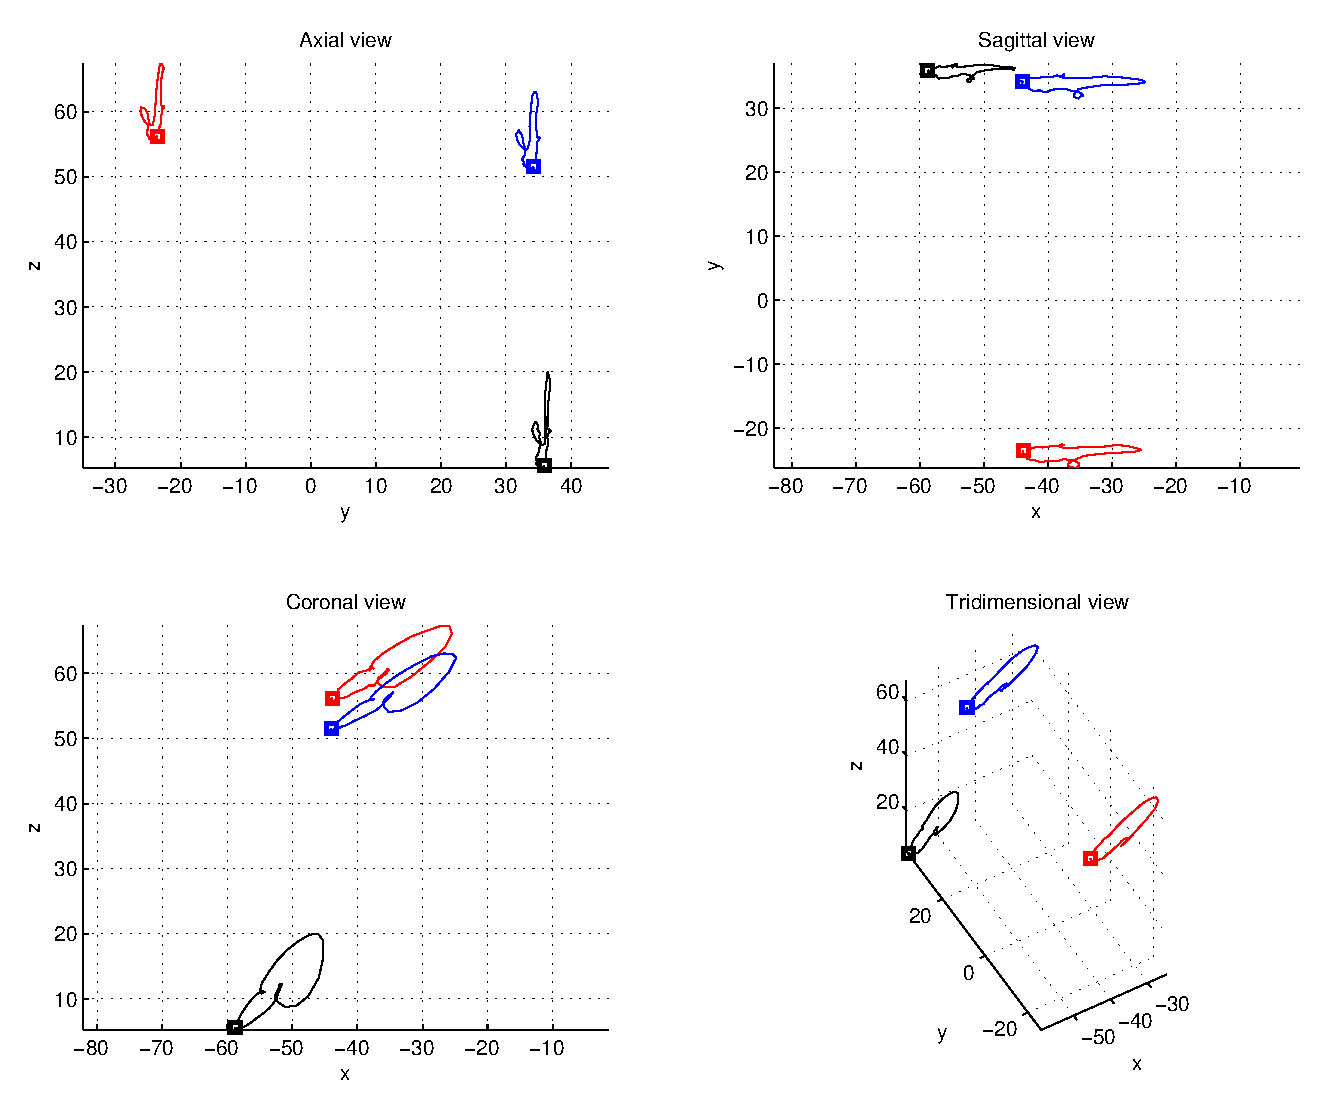
\includegraphics[width=0.45\textwidth]{include/results/images/complex_15_glasses.eps}}
	\hspace{0.05\textwidth}
	\subfigure[\label{fig:results:uovo:complex:tongue}]
	{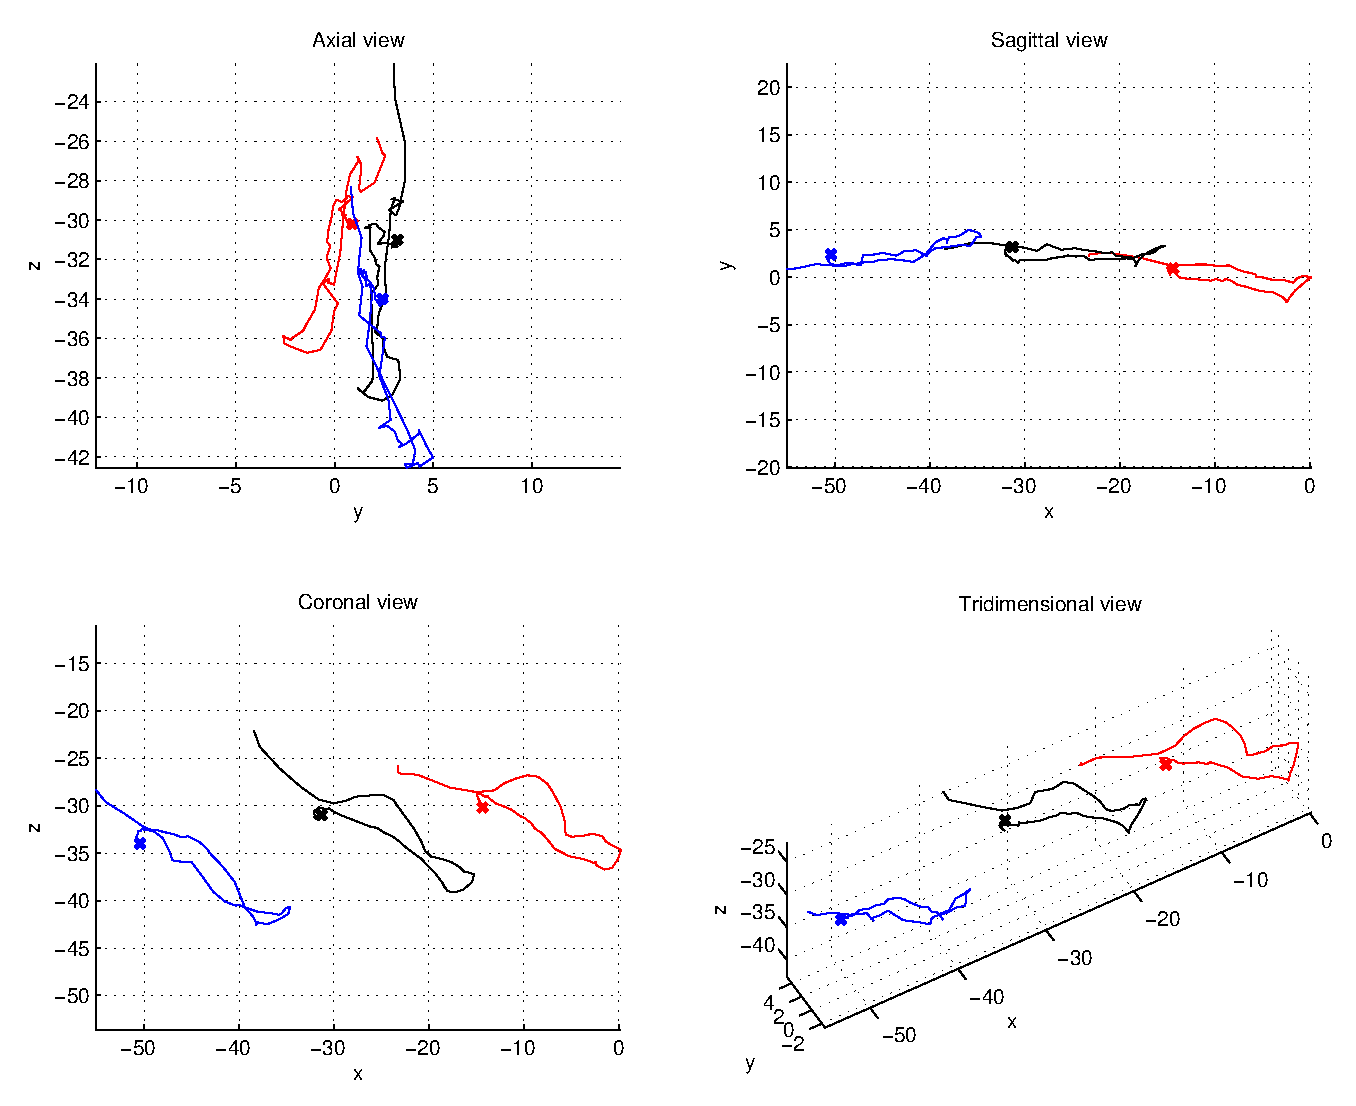
\includegraphics[width=0.45\textwidth]{include/results/images/complex_15_tongue.eps}}

	\caption[Projections of the trajectories of some sensors for 
	/uovo/]{\textbf{Projections of the trajectories of few sensors for /uovo/}: 
	a graphical representation of the trajectories of some sensors is here
	shown for the head-reference sensors (a) and for the three sensors glued 
	sagittally to the dorsum of the tongue (b).
	For each panel (a and b), the axial projection (\emph{yz} plane), 
	the sagittal
	projection (\emph{xy} plane) and the coronal projection (\emph{xz}) are
	shown.
	Furthermore, a tridimensional plot of the trajectories is provided.
	It is important to underline that the subject is looking towards the
	negative direction of the \emph{x} axis.
	Note: (a) sensor 10 in blue, sensor 11 in red and sensor 12 in black; 
	(b) sensor 1 in red, sensor 2 in black and sensor 3 in blue.
	This plot adheres to the convention shown in 
	Figure~\ref{fig:experiments:map}.
	The thick marks indicate the final position of the sensors.
	}
	\label{fig:results:uovo:complex}
\end{figure}
% ---------------------------------------------------------------------------- %
